\documentclass[a5paper, 10pt]{article}

% Текст
\usepackage[utf8]{inputenc} % UTF-8 кодировка
\usepackage[russian]{babel} % Русский язык
\usepackage{indentfirst} % красная строка в первом параграфе в главе
% Отображение страниц
\usepackage{geometry} % размеры листа и отступов
\usepackage{listings}
\usepackage{color}

\geometry{
	left=12mm,
	top=25mm,
	right=15mm,
	bottom=17mm,
	marginparsep=0mm,
	marginparwidth=0mm,
	headheight=10mm,
	headsep=7mm,
	nofoot}
\usepackage{afterpage,fancyhdr} % настройка колонтитулов
\pagestyle{fancy}
\fancypagestyle{style}{ % создание нового стиля style
	\fancyhf{} % очистка колонтитулов
	\fancyhead[LO, RE]{Лабораторная работа № 2 } % название документа наверху
	\fancyhead[RO, LE]{Преобразование Фурье} % название section наверху
	\fancyfoot[RO, LE]{\thepage} % номер страницы справа внизу на нечетных и слева внизу на четных
	\renewcommand{\headrulewidth}{0.25pt} % толщина линии сверху
	\renewcommand{\footrulewidth}{0pt} % толцина линии снизу
}
\fancypagestyle{plain}{ % создание нового стиля plain -- полностью пустого
	\fancyhf{}
	\renewcommand{\headrulewidth}{0pt}
}
\fancypagestyle{title}{ % создание нового стиля title -- для титульной страницы
	\fancyhf{}
	\fancyhead[C]{{\footnotesize
			Министерство образования и науки Российской Федерации\\
			Федеральное государственное автономное образовательное учреждение высшего образования
	}}
	\fancyfoot[C]{{\large 
			Санкт-Петербург, 2024
	}}
	\renewcommand{\headrulewidth}{0pt}
}

% Математика
\usepackage{amsmath, amsfonts, amssymb, amsthm} % Набор пакетов для математических текстов
%\usepackage{dmvnbase} % мехматовский пакет latex-сокращений
\usepackage{cancel} % зачеркивание для сокращений
% Рисунки и фигуры
\usepackage[pdftex]{graphicx} % вставка рисунков
\usepackage{wrapfig, subcaption} % вставка фигур, обтекая текст
\usepackage{caption} % для настройки подписей
\captionsetup{figurewithin=none,labelsep=period, font={small,it}} % настройка подписей к рисункам
% Рисование
\usepackage{tikz} % рисование
\usepackage{circuitikz}
\usepackage{pgfplots} % графики
% Таблицы
\usepackage{multirow} % объединение строк
\usepackage{multicol} % объединение столбцов
% Остальное
\usepackage[unicode, pdftex]{hyperref} % гиперссылки
\usepackage{enumitem} % нормальное оформление списков
\setlist{itemsep=0.15cm,topsep=0.15cm,parsep=1pt} % настройки списков
% Теоремы, леммы, определения...
\theoremstyle{definition}
\newtheorem{Def}{Определение}
\newtheorem*{Axiom}{Аксиома}
\theoremstyle{plain}
\newtheorem{Th}{Теорема}
\newtheorem{Lem}{Лемма}
\newtheorem{Cor}{Следствие}
\newtheorem{Ex}{Пример}
\theoremstyle{remark}
\newtheorem*{Note}{Замечание}
\newtheorem*{Solution}{Решение}
\newtheorem*{Proof}{Доказательство}
% Свои команды
\newcommand{\comb}[1]{\left[\hspace{-4pt}\begin{array}{l}#1\end{array}\right.\hspace{-5pt} } % совокупность уравнений
% Титульный лист
\usepackage{csvsimple-l3}
\newcommand*{\titlePage}{
	\thispagestyle{title}
	\begingroup
	\begin{center}
		%		{\footnotesize
			%			Министерство образования и науки Российской Федерации\\
			%			Федеральное государственное автономное образовательное учреждение высшего образования
			%		}
		%		
		\vspace*{6ex}
		
		{\small
			САНКТ-ПЕТЕРБУРГСКИЙ НАЦИОНАЛЬНЫЙ ИССЛЕДОВАТЕЛЬСКИЙ УНИВЕРСИТЕТ ИТМО	
		}
		
		\vspace*{2ex}
		
		{\normalsize
			Факультет систем управления и робототехники
		}
		
		\vspace*{15ex}
		
		{\Large \bfseries 
			Лабораторная работа № 2
		}
\vspace*{2ex}
	{\Large \bfseries 
			
"Преобразование Фурье"
		}
\vspace*{2ex}
		
		{\normalsize
			по дисциплине Частотные методы
		}

	\end{center}
	\vspace*{20ex}
	\begin{flushright}
		{\large 
			\underline{Выполнила}: студентка гр. \textbf{R3238}\\
			\begin{flushright}
				\textbf{Нечаева А. А.}\\
			\end{flushright}
		}
		
		\vspace*{5ex}
		
		{\large 
			\underline{Преподаватель}: \textit{Перегудин Алексей Алексеевич}
		}
	\end{flushright}	
	\newpage
	\setcounter{page}{1}
	\endgroup}

\begin{document}
	\titlePage
	\pagestyle{style}
\newpage
\textit{В заданиях 1 и 2 используется унитарное преобразование Фурье к угловой частоте} $\omega$.




\section{Задание. Вещественное.}
Все функции ниже $f : \mathbb{R} \to \mathbb{R}$.

\subsection{Прямоугольная функция}

\begin{equation}
f(t) =
\begin{cases}
a, & |t| \leq b,\\
0, & |t| > b
\end{cases}
\end{equation}


\subsubsection{Аналитическое выражение Фурье-образа}

Фурье-образ функции $f(t)$ будем находить по формуле:
\begin{equation}
\hat{f}(\omega) = \frac{1}{\sqrt{2 \pi}} \int \limits_{-\infty}^{\infty} f(t) e^{-i \omega t} dt
\end{equation}



\begin{multline}
\hat{f}(\omega) = \frac{1}{\sqrt{2 \pi}} \int \limits_{-\infty}^{\infty} f(t) e^{-i \omega t} dt = \frac{1}{\sqrt{2 \pi}} \int \limits_{-b}^{b} a e^{-i \omega t} dt =   \frac{a ( e^{-i \omega b} -  e^{i \omega b})}{-i\omega \sqrt{2 \pi}}
\end{multline}

\newpage
\subsubsection{Построение графиков функции $f(t)$}

\begin{figure}[h!]
\center{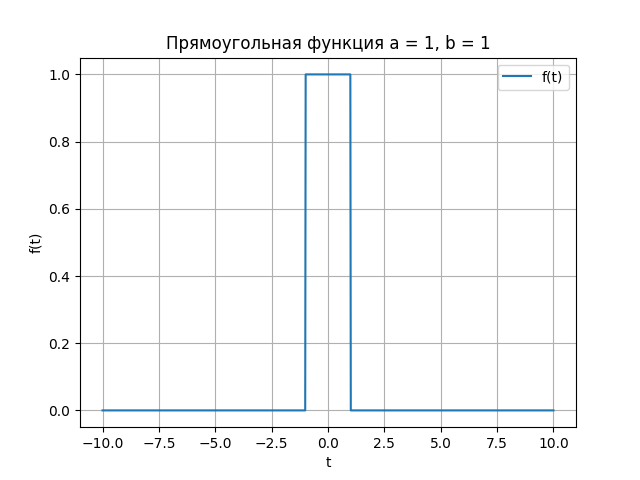
\includegraphics[width=0.76\linewidth]{rect/f_1_1.png}}
\caption{График $f(t)$ при $a = 1$, $b = 1$.}
\center{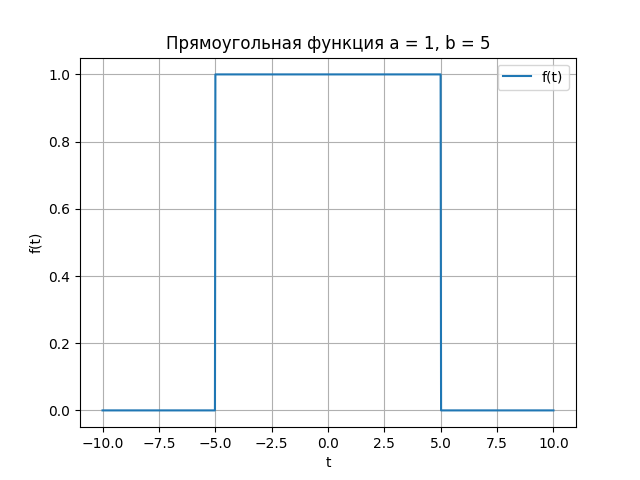
\includegraphics[width=0.76\linewidth]{rect/f_1_5.png}}
\caption{График $f(t)$ при $a = 1$, $b = 5$.}
\end{figure}


\begin{figure}[h!]
\center{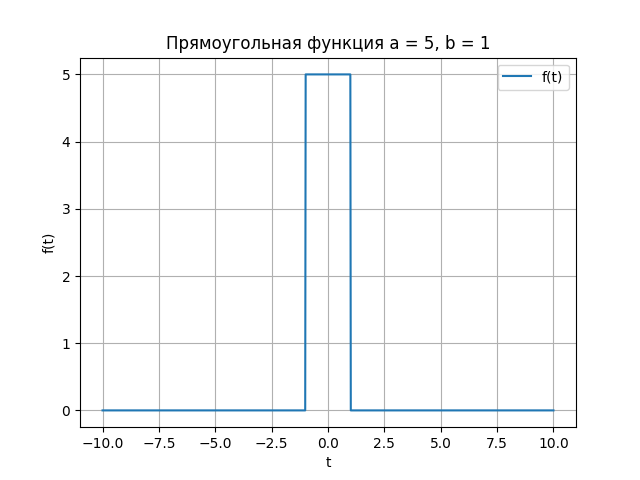
\includegraphics[width=0.76\linewidth]{rect/f_5_1.png}}
\caption{График $f(t)$ при $a = 5$, $b = 1$.}
\center{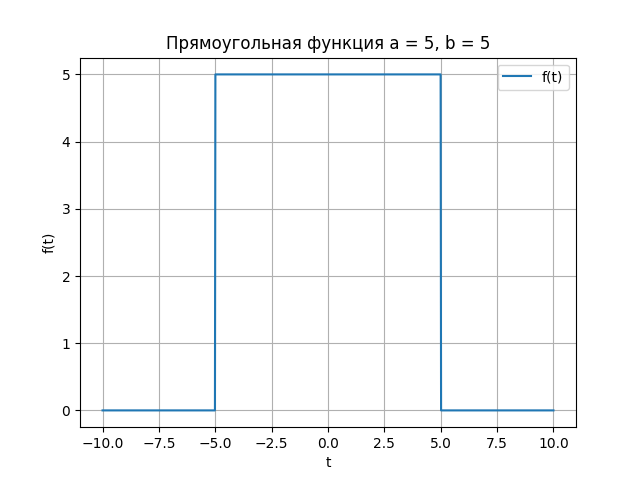
\includegraphics[width=0.76\linewidth]{rect/f_5_5.png}}
\caption{График $f(t)$ при $a = 5$, $b = 5$.}
\end{figure}


\subsubsection{Построение графиков Фурье-образа $\hat{f} (\omega)$}


\begin{figure}[h!]
\center{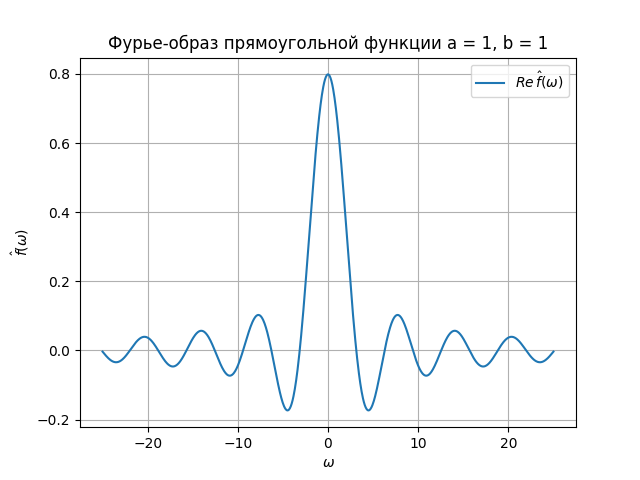
\includegraphics[width=0.75\linewidth]{rect/im_1_1.png}}
\caption{График $\hat{f} (\omega)$ при $a = 1$, $b = 1$.}
\center{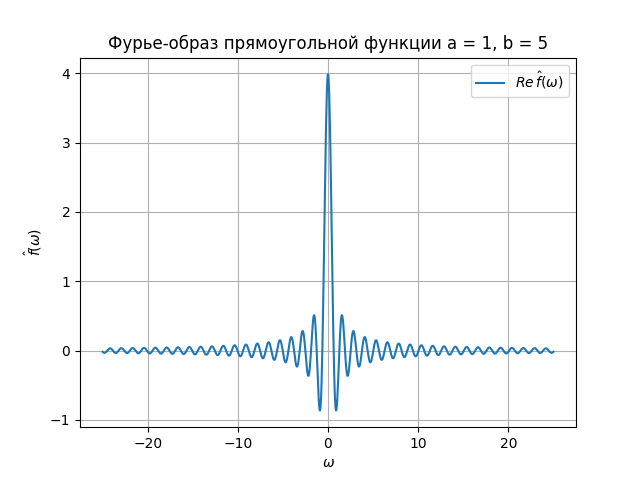
\includegraphics[width=0.75\linewidth]{rect/im_1_5.png}}
\caption{График $\hat{f} (\omega)$ при $a = 1$, $b = 5$.}
\end{figure}


\begin{figure}[h!]
\center{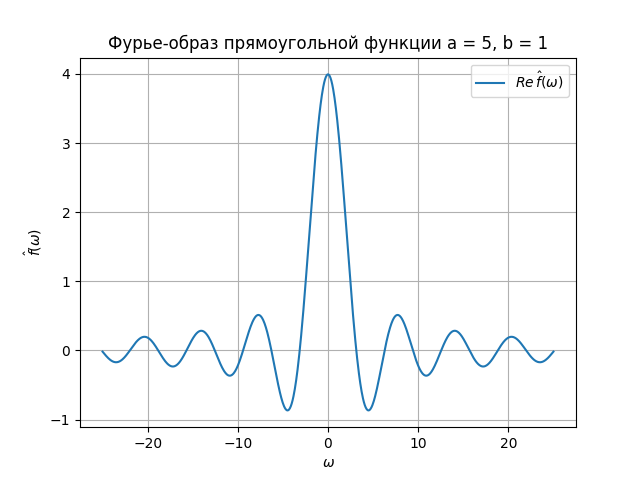
\includegraphics[width=0.76\linewidth]{rect/im_5_1.png}}
\caption{График $\hat{f} (\omega)$ при $a = 5$, $b = 1$.}
\center{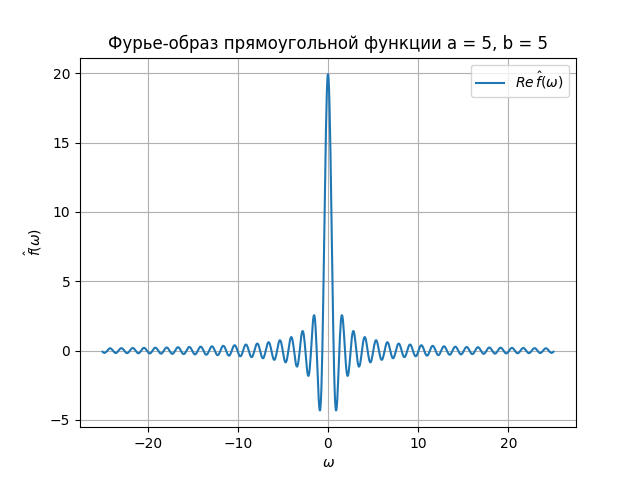
\includegraphics[width=0.76\linewidth]{rect/im_5_5.png}}
\caption{График $\hat{f} (\omega)$ при $a = 5$, $b = 5$.}
\end{figure}



\subsubsection{Проверка равенства Парсеваля}

\begin{table}[h!]
\caption{Равенство Парсеваля для прямоугольной функции.}
\label{tabular:timesandtenses}
\begin{center}
\begin{tabular}{|c|c|c|c|c|}
\hline
n & $a$ & $b$ & $\| f \|^2 = \int_{-d}^d |f(t)|^2 dt $ & $\| \hat{f} \|^2 = \int_{-d}^d |\hat{f}(\omega)|^2 d\omega $ \\
\hline
1 & 1 & 1 &  2.0& 2.0\\
\hline
2 & 1 & 5 &  & \\
\hline
3 & 5 & 1 &  & \\
\hline
4 & 5 & 5 &  & \\
\hline
\end{tabular}
\end{center}
\end{table}







\newpage
\subsection{Треугольная функция}

\begin{equation}
f(t) =
\begin{cases}
a - |at / b|, & |t| \leq b,\\
0, & |t| > b
\end{cases}
\end{equation}


\subsubsection{Аналитическое выражение Фурье-образа}

\begin{multline*}
\hat{f}(\omega) = \frac{1}{\sqrt{2 \pi}} \int \limits_{-\infty}^{\infty} f(t) e^{-i \omega t} dt =
 \frac{1}{\sqrt{2 \pi}} \int \limits_{-b}^{b} (a - |at / b|) e^{-i \omega t} dt =  \frac{1}{\sqrt{2 \pi}} \int \limits_{-b}^{b} a e^{-i \omega t} dt  -\\
- \frac{1}{\sqrt{2 \pi}} \int \limits_{-b}^{b}  |at / b| e^{-i \omega t} dt =   \frac{a ( e^{-i \omega b} -  e^{i \omega b})}{-i\omega \sqrt{2 \pi}} 
+ \frac{a}{b\sqrt{2 \pi}} \left( \int \limits_{-b}^{0}  t e^{-i \omega t} dt -  \int \limits_{0}^{b}  t e^{-i \omega t} dt  \right) \fbox{=}
\end{multline*}

Отдельно вычислим неопределенный интеграл:
\begin{multline}
\int  t e^{-i \omega t} dt = \left|  \right| u = t, \, dv =  e^{-i \omega t} dt, du=dt, v = -\frac{e^{-i \omega t}}{i \omega}\left|  \right| =\\
=  -\frac{t e^{-i \omega t}}{i \omega} + \int \frac{e^{-i \omega t}}{i \omega} dt =  -\frac{t e^{-i \omega t}}{i \omega} + \frac{e^{-i \omega t}}{ \omega^2} + C = \frac{1 + i \omega t}{\omega^2 e^{i \omega t}} + C
\end{multline} 

И два соотвествующих определенных интеграла:
\begin{equation}
\int \limits_{-b}^{0}  t e^{-i \omega t} dt =  \left. \frac{1 + i \omega t}{\omega^2 e^{i \omega t}} \right|^0_{-b} =  \frac{1}{\omega^2} -
 \frac{1 - i \omega b}{\omega^2 e^{-i \omega b}}
\end{equation}

\begin{equation}
\int \limits_{0}^{b}  t e^{-i \omega t} dt =  \left. \frac{1 + i \omega t}{\omega^2 e^{i \omega t}} \right|^b_{0} =
 \frac{1 + i \omega b}{\omega^2 e^{i \omega b}} -\frac{1}{\omega^2} 
\end{equation}

\begin{equation}
\int \limits_{-b}^{0}  t e^{-i \omega t} dt -  \int \limits_{0}^{b}  t e^{-i \omega t} dt  =  \frac{2}{\omega^2} -
 \frac{1 - i \omega b}{\omega^2 e^{-i \omega b}} - \frac{1 + i \omega b}{\omega^2 e^{i \omega b}} 
\end{equation}

\begin{multline}
\fbox{=} \frac{a ( e^{-i \omega b} -  e^{i \omega b})}{-i\omega \sqrt{2 \pi}} + \frac{a}{b\sqrt{2 \pi}} \left( \frac{2}{\omega^2} -
 \frac{1 - i \omega b}{\omega^2 e^{-i \omega b}} - \frac{1 + i \omega b}{\omega^2 e^{i \omega b}}  \right) =\\
=\frac{a}{b \omega^2 \sqrt{2 \pi}} \left( i\omega b (e^{-i \omega b} - e^{i \omega b}) + 2 - e^{i\omega b} + i \omega b e^{i\omega b} - e^{-i\omega b} - i \omega b e^{-i\omega b} \right) = \\
= \frac{a}{b \omega^2 \sqrt{2 \pi}} \left( i\omega b e^{-i \omega b} - i\omega b e^{i \omega b} + 2 - e^{i\omega b} + i \omega b e^{i\omega b} - e^{-i\omega b} - i \omega b e^{-i\omega b} \right) = \\
= \frac{a}{b \omega^2 \sqrt{2 \pi}} \left( 2 - e^{i\omega b}  - e^{-i\omega b} \right) 
\end{multline}


\subsubsection{Построение графиков функции $f(t)$}

\begin{figure}[h!]
\center{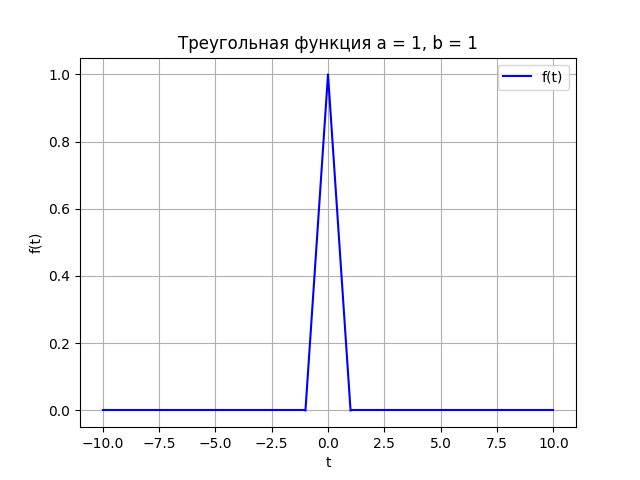
\includegraphics[width=0.76\linewidth]{tria/f_1_1.png}}
\caption{График $f(t)$ при $a = 1$, $b = 1$.}
\end{figure}


\begin{figure}[h!]
\center{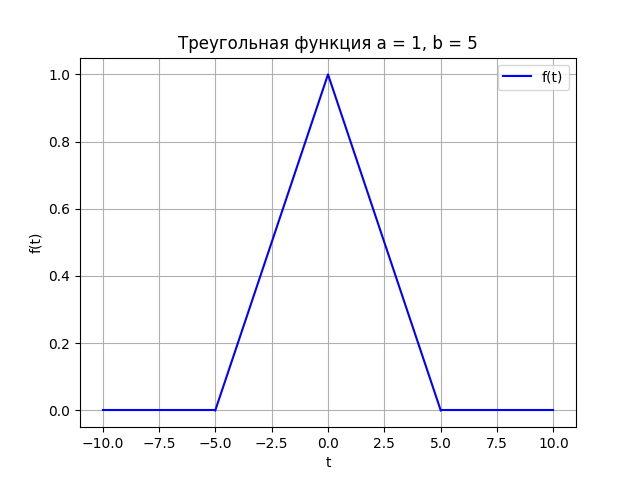
\includegraphics[width=0.76\linewidth]{tria/f_1_5.png}}
\caption{График $f(t)$ при $a = 1$, $b = 5$.}
\center{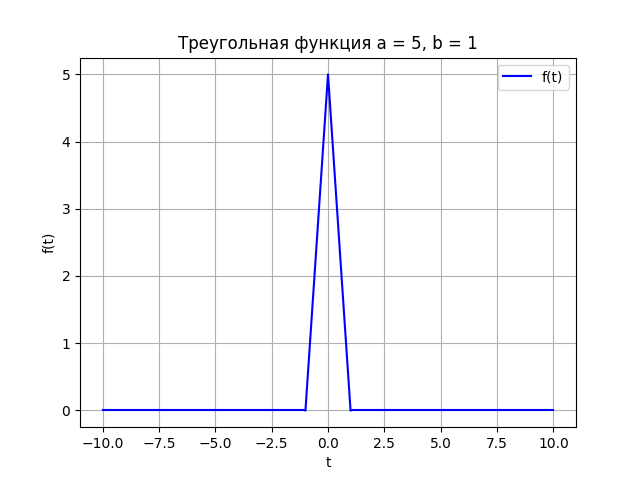
\includegraphics[width=0.76\linewidth]{tria/f_5_1.png}}
\caption{График $f(t)$ при $a = 5$, $b = 1$.}
\end{figure}


\begin{figure}[h!]
\center{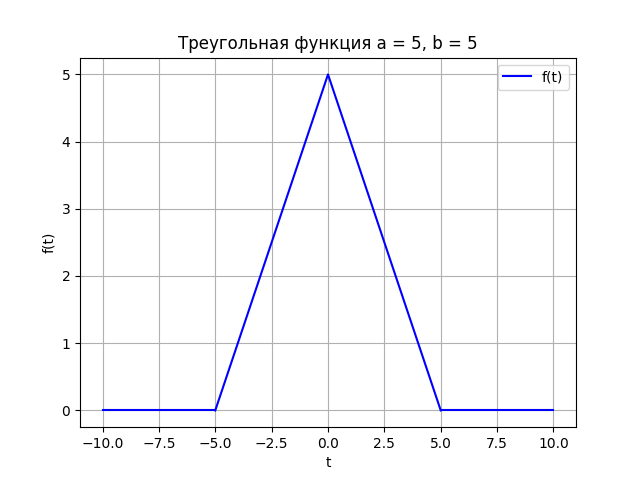
\includegraphics[width=0.76\linewidth]{tria/f_5_5.png}}
\caption{График $f(t)$ при $a = 5$, $b = 5$.}
\end{figure}




\newpage
\subsubsection{Построение графиков Фурье-образа $\hat{f} (\omega)$}



\subsubsection{Проверка равенства Парсеваля}

\begin{table}[h!]
\caption{Равенство Парсеваля для треугольной функции.}
\label{tabular:timesandtenses}
\begin{center}
\begin{tabular}{|c|c|c|c|c|}
\hline
n & $a$ & $b$ & $\| f \|^2 = \int_{-d}^d |f(t)|^2 dt $ & $\| \hat{f} \|^2 = \int_{-d}^d |\hat{f}(\omega)|^2 d\omega $ \\
\hline
1 & 1 & 1 &  2.0& 2.0\\
\hline
2 & 1 & 5 &  & \\
\hline
3 & 5 & 1 &  & \\
\hline
4 & 5 & 5 &  & \\
\hline
\end{tabular}
\end{center}
\end{table}





\newpage
\subsection{Кардинальный синус}
\begin{equation}
f(t) = a sinc(bt)
\end{equation}


\subsubsection{Аналитическое выражение Фурье-образа}

Результат получен с помощью калькулятора $Wolfram$.

\begin{equation}
\hat{f}(\omega) =
 \frac{1}{\sqrt{2 \pi}} \int \limits_{-\infty}^{\infty}  a sinc(bt) e^{-i \omega t} dt = 
 \frac{a}{|b|} \sqrt{\frac{\pi}{2}} \cdot
\begin{cases}
0, & \left( \frac{b}{\omega} \right)^2 \leq 1\\
1 & (otherwise)
\end{cases}
\end{equation}


\subsubsection{Построение графиков функции $f(t)$}






\subsubsection{Построение графиков Фурье-образа $\hat{f} (\omega)$}





\subsubsection{Проверка равенства Парсеваля}

\begin{table}[h!]
\caption{Равенство Парсеваля для кардинального синуса.}
\label{tabular:timesandtenses}
\begin{center}
\begin{tabular}{|c|c|c|c|c|}
\hline
n & $a$ & $b$ & $\| f \|^2 = \int_{-d}^d |f(t)|^2 dt $ & $\| \hat{f} \|^2 = \int_{-d}^d |\hat{f}(\omega)|^2 d\omega $ \\
\hline
1 & 1 & 1 &  2.0& 2.0\\
\hline
2 & 1 & 5 &  & \\
\hline
3 & 5 & 1 &  & \\
\hline
4 & 5 & 5 &  & \\
\hline
\end{tabular}
\end{center}
\end{table}






\newpage
\subsection{Функция Гаусса}

\begin{equation}
f(t) = a e^{-bt^2}
\end{equation}


\subsubsection{Аналитическое выражение Фурье-образа}

Результат получен с помощью калькулятора $Wolfram$.

\begin{equation}
\hat{f}(\omega) =
 \frac{1}{\sqrt{2 \pi}} \int \limits_{-\infty}^{\infty}  a e^{-bt^2} e^{-i \omega t} dt = \frac{a}{\sqrt{2b}} e^{-\frac{\omega^2}{4b}}
\end{equation}

\subsubsection{Построение графиков функции $f(t)$}





\subsubsection{Построение графиков Фурье-образа $\hat{f} (\omega)$}




\subsubsection{Проверка равенства Парсеваля}

\begin{table}[h!]
\caption{Равенство Парсеваля для функции Гаусса.}
\label{tabular:timesandtenses}
\begin{center}
\begin{tabular}{|c|c|c|c|c|}
\hline
n & $a$ & $b$ & $\| f \|^2 = \int_{-d}^d |f(t)|^2 dt $ & $\| \hat{f} \|^2 = \int_{-d}^d |\hat{f}(\omega)|^2 d\omega $ \\
\hline
1 & 1 & 1 &  2.0& 2.0\\
\hline
2 & 1 & 5 &  & \\
\hline
3 & 5 & 1 &  & \\
\hline
4 & 5 & 5 &  & \\
\hline
\end{tabular}
\end{center}
\end{table}






\newpage
\subsection{Двустороннее затухание}

\begin{equation}
f(t) = a e^{-b|t|}
\end{equation}


\subsubsection{Аналитическое выражение Фурье-образа}

\begin{multline}
\hat{f}(\omega) =
 \frac{1}{\sqrt{2 \pi}} \int \limits_{-\infty}^{\infty} a e^{-b|t|} e^{-i \omega t} dt =  \frac{a}{\sqrt{2 \pi}}  \left( \int \limits_{-\infty}^{0} e^{b t} e^{-i \omega t} dt  + \int \limits_{0}^{\infty} e^{-b t} e^{-i \omega t} dt  \right) = \\
=  \frac{a}{\sqrt{2 \pi}}  \left( \int \limits_{-\infty}^{0} e^{(b-i \omega) t} dt  + \int \limits_{0}^{\infty}e^{-(b + i \omega) t} dt  \right) 
= \frac{a}{\sqrt{2 \pi}}  \left(  \left. \frac{e^{(b-i \omega) t}}{b-i \omega} \right|_{-\infty}^{0} + \left. \frac{e^{-(b + i \omega) t}}{-(b + i \omega)} \right|_{0}^{\infty}  \right) =\\
=\frac{a}{\sqrt{2 \pi}}  \left( \frac{1}{b-i \omega} + \frac{1}{b + i \omega}  \right) =
\frac{a}{\sqrt{2 \pi}}   \frac{b + i \omega +b - i \omega}{b^2 + \omega^2} = \frac{2ab}{\sqrt{2 \pi} (b^2 + \omega^2)}
\end{multline}

\subsubsection{Построение графиков функции $f(t)$}




\subsubsection{Построение графиков Фурье-образа $\hat{f} (\omega)$}



\subsubsection{Проверка равенства Парсеваля}

\begin{table}[h!]
\caption{Равенство Парсеваля для двустороннего затухания.}
\label{tabular:timesandtenses}
\begin{center}
\begin{tabular}{|c|c|c|c|c|}
\hline
n & $a$ & $b$ & $\| f \|^2 = \int_{-d}^d |f(t)|^2 dt $ & $\| \hat{f} \|^2 = \int_{-d}^d |\hat{f}(\omega)|^2 d\omega $ \\
\hline
1 & 1 & 1 &  2.0& 2.0\\
\hline
2 & 1 & 5 &  & \\
\hline
3 & 5 & 1 &  & \\
\hline
4 & 5 & 5 &  & \\
\hline
\end{tabular}
\end{center}
\end{table}





Для визуализации был написан код на языке \textit{Python}. \\
Код расположен на \href{https://github.com/a-nechaeva/practical_Linal/tree/main/lab4}{\textbf{GitHub}}.
\end{document}













